\setcounter{chapter}{16}
\exam{Teste 1 2016/17}
\question{Pergunta 1}
\textbf{(a)} O método da bisecção implica encontrar um intervalo inicial $[a,b]$ ao qual pertença a raiz da função, que, apesar de bastante simples, consegue ser mais complexo do que utilizar o método de Picard-Peano, que neste Pergunta corresponde a encontrar a única recorrência possível
\begin{gather*}
	\frac{Bx-1}{x-1}=0 \iff Bx-1=0 \iff x=\frac{1}{B}\\
	x_{n+1}=\frac{1}{B}
\end{gather*}
e aplicá-la uma única vez, dado que esta solução pelo método de Picard-Peano corresponde também à solução algébrica, para os valores de $B$ em que a equação do enunciado é válida ($B\neq 0 \wedge B\neq 1$).\\
\textbf{(b)}
\lstinputlisting[language=C++, caption=Código-fonte 2016T1-1 (C++)]{01.cpp}
\begin{center}
\begin{tabular}{ p{73mm} p{0mm} p{73mm} }
	\lstinputlisting[caption=Input 2016T1-1]{01.in} & &
	\lstinputlisting[caption=Output 2016T1-1]{01.out}
\end{tabular}
\end{center}

\question{Pergunta 3}
\questionitem{Item a}
Espero encontrar duas soluções, uma próxima de $(-1.2,-0.6)$ e outra próxima de $(0.2,1)$.

\newpage
\questionitem{Item b}
\begin{equation*}
	\begin{cases}
		f_1(x,y)=0.7+x-y\\
		f_2(x,y)=1-x^2-y
	\end{cases}
	\implies
	\mathbf{J}=\begin{bmatrix}
  		f_{1,x}' & f_{1,y}'\\
  		f_{2,x}' & f_{2,y}'
	\end{bmatrix}=\begin{bmatrix}
  		1   & -1\\
  		-2x & -1
	\end{bmatrix}
	\implies
	|\mathbf{J}|=-2x-1
\end{equation*}
\begin{alignat*}{4}
	h&=-\frac{
		\begin{vmatrix}
			f_1 & f_{1,y}' \\
			f_2 & f_{2,y}'
		\end{vmatrix}}
		{|\mathbf{J}|}
	   &&=-\frac{
		\begin{vmatrix}
			0.7+x-y & -1 \\
			1-x^2-y & -1
		\end{vmatrix}}
		{|\mathbf{J}|}
	   &&=-\frac{-x^2-x+0.3}{-2x-1}
	   &&=-\frac{x^2+x-0.3}{2x+1} \\
	k&=-\frac{
		\begin{vmatrix}
			f_{1,x}' & f_1 \\
			f_{2,x}' & f_2
		\end{vmatrix}}
		{|\mathbf{J}|}
	   &&=-\frac{
		\begin{vmatrix}
			 1  & 0.7+x-y \\
			-2x & 1-x^2-y
		\end{vmatrix}}
		{|\mathbf{J}|}
	   &&=-\frac{x^2+1.4x-y-2x y+1}{-2x-1}
	   &&=\frac{x^2+1.4x-y-2x y+1}{2x+1}
\end{alignat*}
\begin{equation*}
	\begin{cases}
		x'=x+h\\
		y'=y+k
	\end{cases}
	\iff
	\begin{cases}
		x'=x-\dfrac{x^2+x-0.3}{2x+1}\\[1em]
		y'=y+\dfrac{x^2+1.4x-y-2x y+1}{2x+1}
	\end{cases}
	\iff
	\begin{cases}
		x'=\dfrac{x^2+0.3}{2x+1}\\[1em]
		y'=\dfrac{x^2+1.4x+1}{2x+1}
	\end{cases}
\end{equation*}
Para avaliar a condição de convergência, já colocámos as recorrências da equação anterior na forma necessária
\begin{equation*}
	\begin{cases}
		x_{n+1}=g_1(x_n,y_n)\\
		y_{n+1}=g_2(x_n,y_n)
	\end{cases}\\
\end{equation*}
\begin{alignat*}{6}
	g_{xx}
	&=&&\left|\frac{\partial g_1}{\partial x}\right|&&+\left|\frac{\partial g_2}{\partial x}\right|
	&&=\left|\frac{2x}{2x+1}-\frac{2x^2+0.6}{(2x+1)^2}\right|&&+\left|\frac{2x^2+2.8x+2}{(2x+1)^2}-\frac{2x+1.4}{2x+1}\right|\\
	g_{yy}
	&=&&\left|\frac{\partial g_1}{\partial y}\right|&&+\left|\frac{\partial g_2}{\partial y}\right|
	&&=\left|0\right|&&+\left|0\right|
	&&=0\\
	g_{xy}
	&=&&\left|\frac{\partial g_1}{\partial x}\right|&&+\left|\frac{\partial g_2}{\partial y}\right|
	&&=\left|\frac{2x}{2x+1}-\frac{2x^2+0.6}{(2x+1)^2}\right|&&+\left|0\right|
	&&=\left|\frac{2x}{2x+1}-\frac{2x^2+0.6}{(2x+1)^2}\right|\\
\end{alignat*}
Procedi à visualização de $g_{xx}$, $g_{yy}$ e $g_{xy}$ em gráfico com $x$ como única variável independente, uma vez que $y$ não influencia o valor de qualquer das funções.
\begin{center} 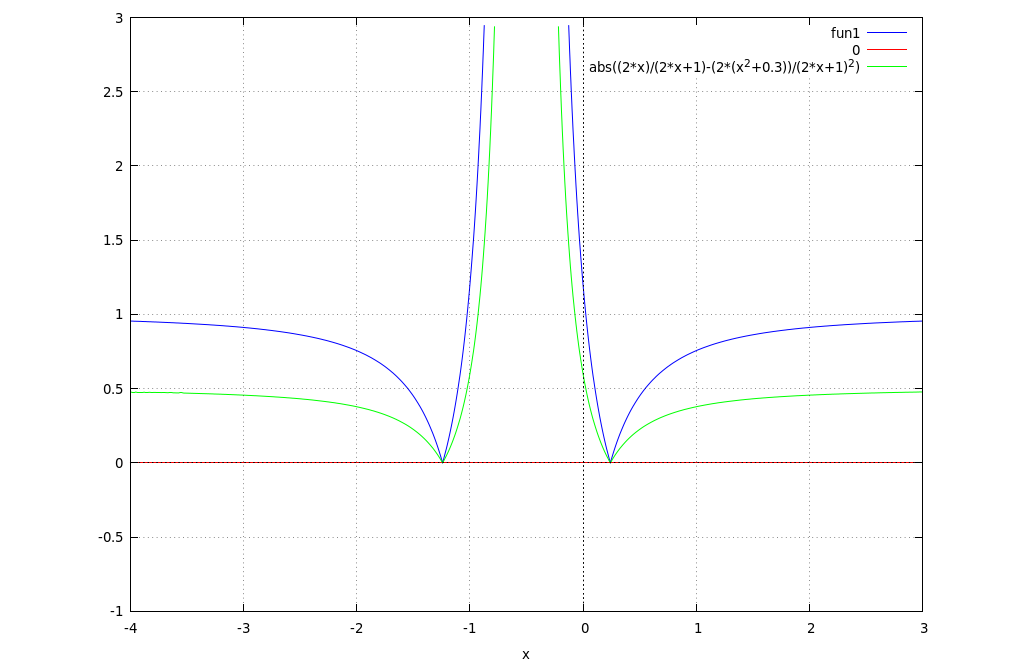
\includegraphics[height=65mm,keepaspectratio]{plots2016T1-3c} \end{center}
Pode-se provar que, para valores $x<-1.1$ e $0.1<x$, as funções possuem todas ordenadas inferiores a $1$, mas o gráfico é suficientemente esclarecedor quanto a essa questão.\\
Assim, se $x<-1.1\wedge y\in\mathbb{R}$ ou se $0.1<x \wedge y\in\mathbb{R}$, pela condição de convergência o processo converge.\\
Escolhi o par ordenado $(x,y)=(-2,0)$, por se encontrar dentro da primeira gama de valores de $x$ para os quais o processo converge.\\

\questionitem{Item c}
\lstinputlisting[language=C++, caption=Código-fonte 2016T1-3c (C++)]{03_c.cpp}
\begin{center}
\begin{tabular}{ p{73mm} p{0mm} p{73mm} }
	\lstinputlisting[caption=Input 2016T1-3c]{03_c.in} & &
	\lstinputlisting[caption=Output 2016T1-3c]{03_c.out}
\end{tabular}
\end{center}

\newpage
\questionitem{Item d}
\begin{center}
\begin{tabular}{ p{73mm} p{0mm} p{73mm} }
	\begin{equation*}
		\begin{cases}
			x_{n+1}=-\sqrt{1-y_n}\\
			y_{n+1}=0.7+x_n
		\end{cases}
	\end{equation*} & &
	\begin{equation*}
		\begin{cases}
			x_{n+1}=-y_n-0.7\\
			y_{n+1}=1-x_n^2
		\end{cases}
	\end{equation*} \\
	\lstinputlisting[language=C++, caption=Código-fonte 2016T1-3di (C++)]{03_di.cpp} & &
	\lstinputlisting[language=C++, caption=Código-fonte 2016T1-3dii (C++)]{03_dii.cpp} \\
\end{tabular}
\end{center}
\lstinputlisting[caption=Input 2016T1-3d]{03_d.in}
\newpage
\begin{center}
\begin{tabular}{ p{73mm} p{0mm} p{73mm} }
	\lstinputlisting[caption=Output 2016T1-3di,basicstyle=\small]{03_di.out} & &
	\lstinputlisting[caption=Output 2016T1-3dii,basicstyle=\small]{03_dii.out}
\end{tabular}
\end{center}
Como é evidente pelos resultados, ambos os conjuntos de expressões recorrentes convergiram para soluções, se bem que para soluções diferentes:
\begin{itemize}
	\item (I) para $(-1.24161984870956620952142657188233, -0.54161984870956625393034755688859)$;
	\item (II) para $(+0.24161984870956626503257780314016, +0.94161984870956627613480804939172)$;
\end{itemize}
Apesar de ambos os métodos convergirem com velocidade comparável, inicialmente o método (II) parece convergir ligeiramente mais depressa até à iteração $26$, quando parece que o método (I) ganha um pequeno avanço, sendo que a diferença entre iterações consecutivas se torna indiscernível para o método (I) à iteração 83, e para o método (II) à iteração 100.\\
De entre as operações utilizadas, $\sqrt{}$ é a que confere menor segurança em termos de implementação, sugerindo que o método (I) pode não ser tão confiável como o método (II) por utilizar $\sqrt{}$.\\
As soluções exatas em $x$ são as soluções da equação
\begin{equation*}
	x^2+x-0.3=0
	\iff x=\frac{-1\pm\sqrt{1^2-4*1*(-0.3}}{2*1}
	\iff x=\frac{-1\pm\sqrt{2.2}}{2}
\end{equation*}
que, por Python3, dão os pares $(x,y)$ com os valores:
\begin{itemize}
	\item $(x_1,y_1)=(-1.24161984870956632481162816431227,-0.54161984870956632481162816431227)$
	\item $(x_2,y_2)=(0.24161984870956632481162816431227,0.94161984870956632481162816431227)$
\end{itemize}
Os erros absolutos na última iteração são
\begin{itemize}
	\item em (I), $\varepsilon_x=\num{2.22E-16}$ e $\varepsilon_y=\num{1.11E-16}$
	\item em (II), $\varepsilon_x=\num{5.55E-17}$ e $\varepsilon_y=\num{4.87E-17}$ 
\end{itemize}
que são compreensivelmente resultado do limite de precisão do double em C++ (até porque o nosso critério de paragem é a indescirnibilidade entre iterações consecutivas, que se verifica em computadores como consequência do limite da representação de números).\\
Os erros absolutos na 40ª iteração são
\begin{itemize}
	\item em (I), $\varepsilon_x=\num{1.98E-8}$ e $\varepsilon_y=\num{6.80E-8}$
	\item em (II), $\varepsilon_x=\num{3.89E-8}$ e $\varepsilon_y=\num{6.22E-8}$ 
\end{itemize}
o que também suporta o facto de que (I) converge mais rapidamente que (II), uma vez que $y$ depende apenas de $x$, $x$ depende de si próprio e o erro absoluto à 40ª iteração em $x$ é menor em (I) do que em (II).